% Overview 
To solve the problem of performing efficient searchs on spatial data, 
Guttman proposed the R-tree, which inspired a variety of different 
variations analagous to the family of B-trees. In Section~\ref{sec:rtrees}
we describe the original R-tree, and in Section~\ref{sec:variants}
we examine the variants and draw appropriate comparisons.

\subsection{R-Trees}
\label{sec:rtrees}
In 1984, Guttman first proposed the idea of modifying the B-tree structure to
use minimum bounding rectangles (MBR) as a way to restrict the search space 
during a lookup for spatial data\cite{guttman84}. Before this, spatial data was
represented using structures such as Quad trees\cite{} and k-d trees\cite{}.

The data structure that resulted from Guttman's research
was called the R-tree. R-trees are structured similarly to B-trees except, instead 
of having separation values in each internal node that divide its subtrees, R-tree 
internal node entries correspond to MBRs that bound its descendents. 
Figure~\ref{fig:R-Tree_structure} shows the R-tree representation for the objects 
of Figure~\ref{fig:R-Tree_objects}. As we observe, the MBR of a particular node 
completely overlaps the MBRs of the nodes of its child and its child's children. 
Like in the B-tree case, nodes correspond to disk pages and leaves point to 
database objects.

\begin{figure}[t]
	\begin{subfigure}{0.48\textwidth}
		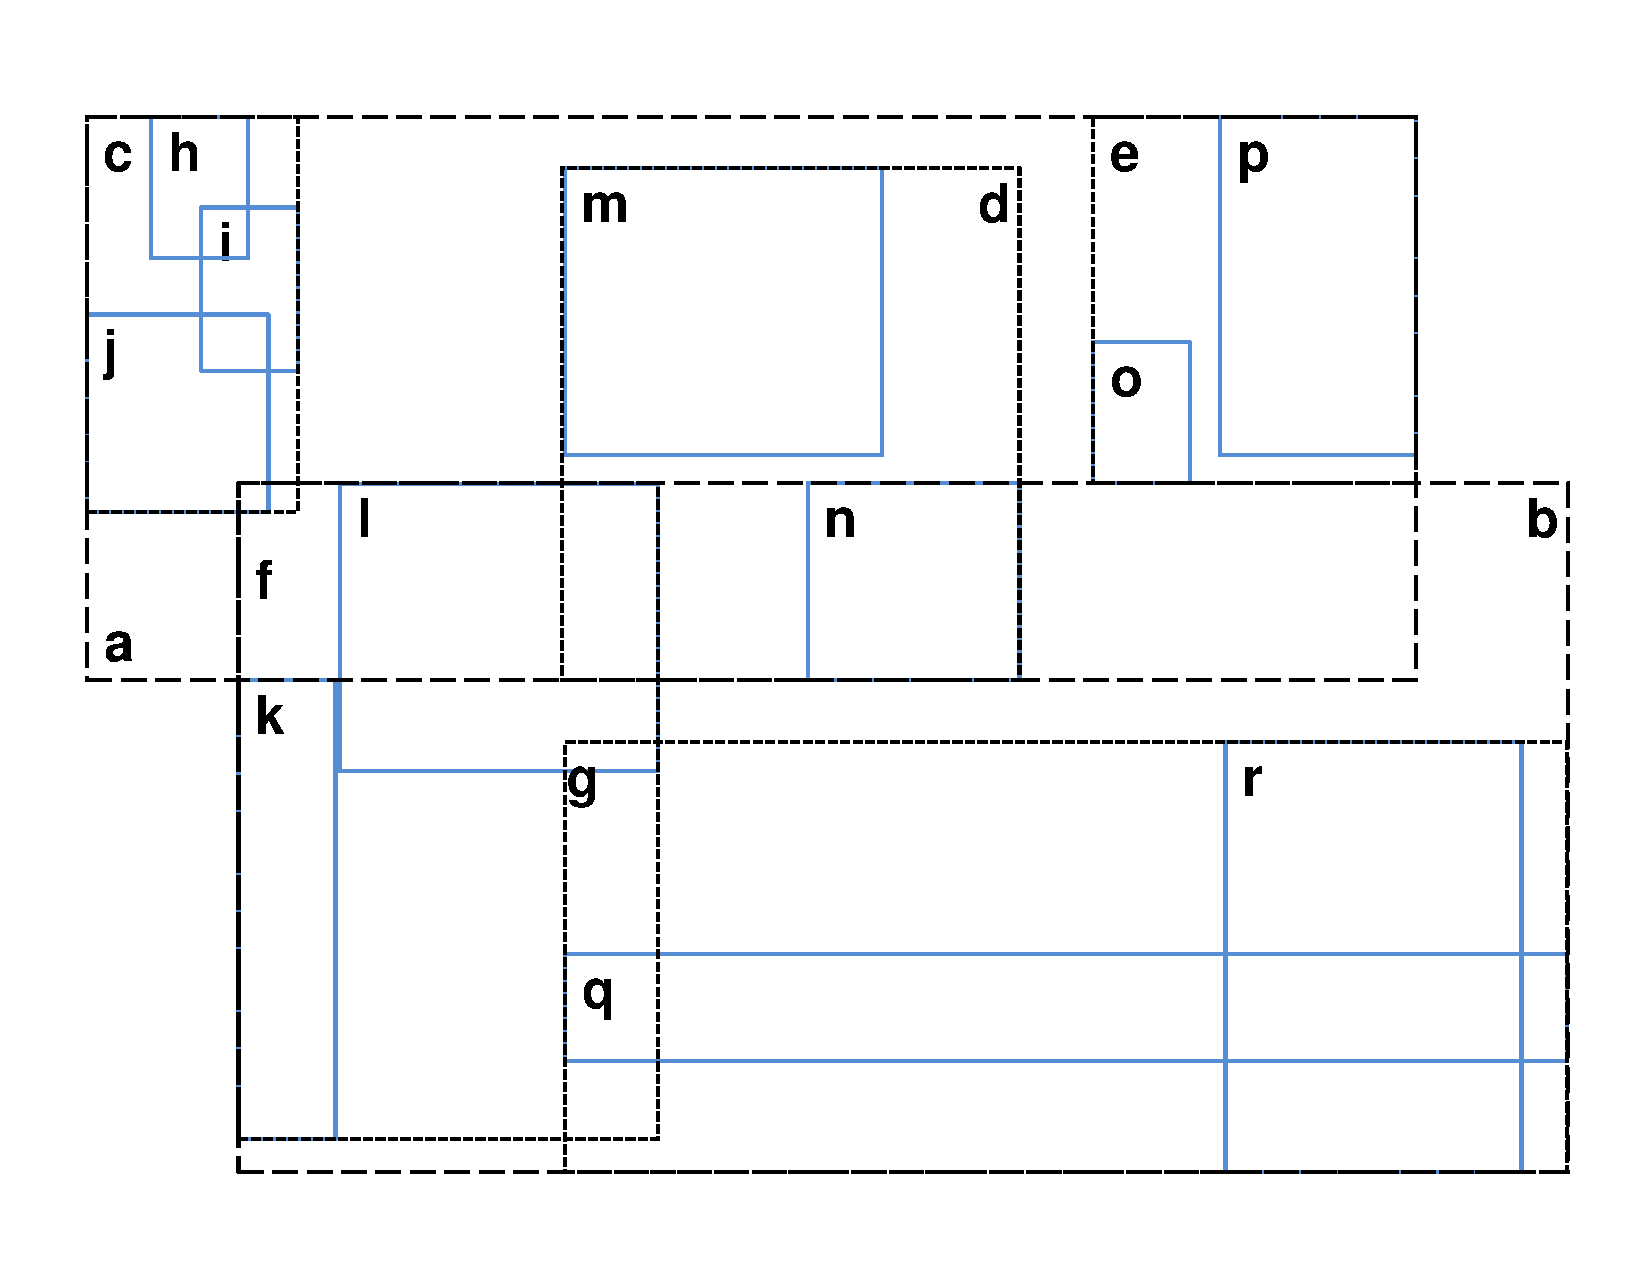
\includegraphics[width=\textwidth]{./figures/R_Tree_objects.pdf}
		\caption{Spatial objects bounded by MBRs}
		\label{fig:R-Tree_objects}
	\end{subfigure}
	~
	\begin{subfigure}{0.48\textwidth}
		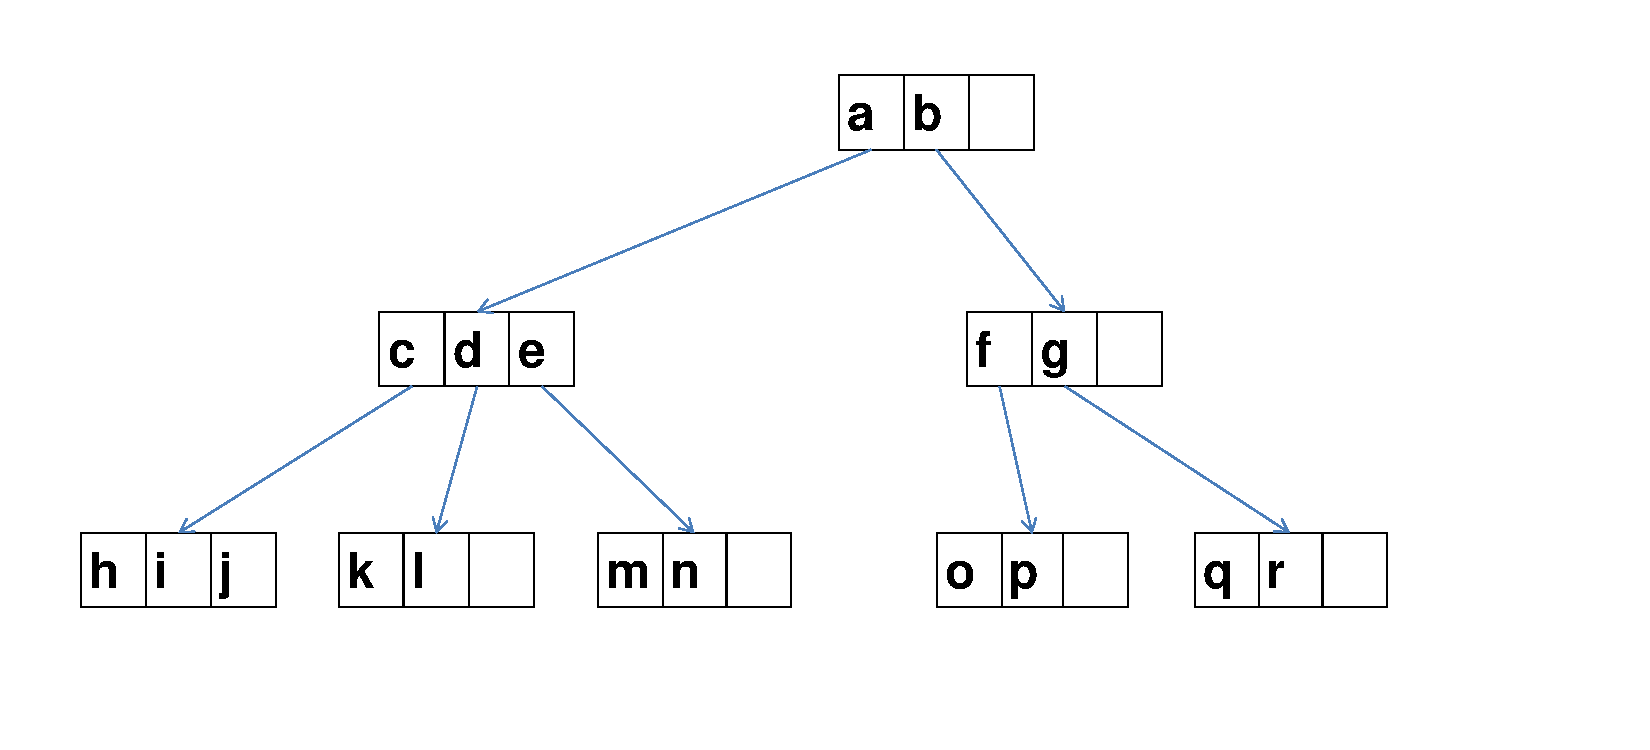
\includegraphics[width=\textwidth]{./figures/R_Tree_structure.pdf}
		\caption{R-tree structure for the objects of part a}
		\label{fig:R-Tree_structure}
	\end{subfigure}
	\caption{Spatial data and corresponding R-tree structure}
\end{figure}


R-trees are bound by two parameters $m$ and $M$, the minimum and maximum number
of entries for each node except the root, respectively. An internal node entry 
is of the form ($mbr$, $p$), where $mbr$ is the MBR containing the MBRs of its 
descendents and $p$ is the pointer to its child subtree. The $mbr$ entry is of 
the form ($I_{0}$, $I_{1}$, ..., $I_{n-1}$), where $n$ is the number of 
dimensions and $I_{i}$ is of form $[a$,$b]$, a closed bounded interval along 
the i-th dimension. Similarly, a leaf node entry is of the form ($mbr$, $oid$), 
where $mbr$ is the MBR containing the object, and oid is the identifier for the 
object in the database. Finally, the root node must have at least three entries
except if it is a leaf.

There are multiple operations that are associated with an R-tree, which we 
discuss in the following sections.

\subsubsection{Search and Update}
In order to find all entries overlapped by a bounding rectangle $S$ in the 
R-tree, the pseudocode of Figure~\ref{fig:R_Tree_Search} is used. In a similar 
fashion to a B-tree traversal, each node in the tree starting from the root is 
checked for overlap using the $mbr$ field in the entry. If there is overlap, 
the search descends into the subtree pointed to by $p$ until it reaches a leaf. 
If the leaf entry's $mbr$ overlaps with $S$, then the object ID $oid$ is 
returned. Note that there is no worst-case performance guarantee for this
algorithm.

Updates are slightly more complex. If a tuple is changed such that the MBR
covering it is also changed, its record in the R-tree must be deleted and then
reinserted. This makes the cost of an update relatively expensive.

\begin{figure}[t]
\begin{algorithmic}
	\Function{Search}{$T$, $S$}
		\If{$T$ is not a leaf}
			\ForAll{$E$ in $T$}
				\If{$E.mbr$ overlaps $S$}
					\State \Call{Search}{$E.p$, $S$}
				\EndIf
			\EndFor
		\Else
			\ForAll{$E$ in $T$}
				\If{$E.mbr$ overlaps $S$}
					\Return $E.oid$
				\EndIf
			\EndFor
		\EndIf
	\EndFunction
\end{algorithmic}
\caption{Pseudocode for finding all entries in a R-tree rooted at T overlapped 
	by a search rectangle S}
\label{fig:R_Tree_Search}
\end{figure}

\subsubsection{Insert}
Insertion again is similar to B-tree insertion methods, as illustrated by the 
algorithm in Figure~\ref{fig:R_Tree_Insert}. The algorithm traverses the tree 
to find the appropriate node to insert into and performs splits when inserting
into full nodes, but there is one important distinction: node splitting 
heuristics. B-tree node splitting is simple since it is only necessary to 
partition the two resulting nodes into two equally sized nodes. In R-trees, the 
goal typically is to create two nodes such that it is unlikely for both to be
examined on subsequent searches by minimizing the total area of the MBRs for
both nodes.

In the original R-tree paper, Guttman discusses three different types of node 
splitting algorithms of different complexities: linear, quadratic, and 
exponential. The linear split algorithm is the most lightweight, but may
result in suboptimal splits since it does not perform an exhaustive search on
all possible groupings. It divides a group of entries into two groups by first 
selecting two seed entries to be the first entries in each group. The two 
entries with the highest normalized separation along any dimension are chosen.
Of the remaining entries, a random one is chosen and placed in the group that 
would have the least enlargement. The exception is if the number of remaining 
entries plus the number of entries in one group is equal to $m$, the minimum 
number of entries in a node, all remaining entries are put into that group. 

The quadratic split algorithm is identical to the linear algorithm, except the 
entries chosen to be seeds are the ones with that have the most wasted space
if grouped together; in other words, the two entries that have the maximum $d$
where $d = area(MBR_{i,j}) - area(E_{i}) - area(E_{j}) $.
Also, the way the remaining entries are added is different than the linear 
algorithm. In this case, the area increase for both groups is calculated for each
entry, and the entry with the maximum difference between the two will be inserted 
into the group that will result in less enlargement.

The exponential split algorithm is an exhaustive search that enumerates all possible
groupings for the entries. Given an R-tree with $M$, the maximum number of entries
in a node, the search space for this algorithm is on the order of $2^{M-1}$.

\begin{figure}[t]
\begin{algorithmic}
	\Function{Insert}{$T$, $E$}
		\State \Call{ChooseLeaf}{$T$, $E$}
		\Comment{Traverse tree from $T$ to appropriate leaf.
			At each level choose node $L$ whose MBR will
			need the least enlargement to cover E.mbr or
			if there is a tie, choose node with minimum
			area. Return $L$
		}
		\If{$L$ is not full}
			\State Insert $E$ into $L$
		\Else
			\State \Call{SplitNode}{$L$}
			\Comment{Returns $L$ and $LL$ containing $E$ and the old
				entries of $L$}
		\EndIf
		\State \Call{AdjustTree}{$L$}
		\Comment{Ascend from leaf node $L$ up to the root $T$
			and propagate splits. }
	\EndFunction
\end{algorithmic}
\caption{Pseudocode for inserting into an R-tree rooted at T given an entry E}
\label{fig:R_Tree_Insert}
\end{figure}

\subsubsection{Delete}
Deletion is handled by the algorithm of Figure~\ref{fig:R_Tree_Delete}. First,
we find the leaf containing the entry to be deleted. Then, we handle the case
where nodes are underfull by calling $CondenseTree$ on the leaf that held
the entry. Instead of merging the underfull node with a sibling like in a 
B-tree, the node is deleted, the other nodes in the leaf are reinserted into 
the R-tree, and the ancestor MBRs are adjusted accordingly. Guttman argues that
reinsertion has two advantages; first, it is easier to implement, and second, 
it prevents deterioration of the R-tree. We will see in other implementations
of the R-tree that this is not the only strategy for deletion.

\begin{figure}[t]
\begin{algorithmic}
\Function{Delete}{$T$, $E$}
	\State \Call{FindLeaf}{$T$, $E$}
	\Comment{Traverse tree from $T$ to appropriate leaf.
			Return node $L$ containing $E$}
	\State Delete $E$ from $L$
	\State \Call{CondenseTree}{$L$}
	\Comment{Given leaf $L$ where $E$ was deleted, if $L$ was
	underfull, reinsert other entries in $L$, delete, and propagate changes
	upward}
\EndFunction
\end{algorithmic}
\caption{Pseudocode for deleting an entry E from an R-tree rooted at T}
\label{fig:R_Tree_Delete}
\end{figure}

\subsection{R-Tree Variants}
\label{sec:variants}
At the time, the R-tree  was a great solution to the problem of efficiently searching
for spatial data in a database; however, there were certain issues with the original
implementation. For instance, the complexity of the insertion algorithm
depends on the complexity of the node splitting function, which is typically
quadratic. Similarly, the heuristics for node splitting affects the efficiency of 
the search algorithm. These challenges are discussed in detail in 
Section~\ref{sec:impchal}. In the below sections, we discuss the main R-Tree
variants that seek to solve some of the disadvantages of the R-tree.

\subsubsection{$R^{+}$-Trees}
Shortly after Guttman's paper in 1984, Sellis, Roussopoulos, and Faloutsos proposed 
the $R^{+}$-tree. The problem they sought to solve was the performance degredation 
during a range search due to high MBR overlap. Basically, the $R^{+}$-tree tries to 
reduce the number of paths explored (and consequently the number of I/O operations) 
during a search by disallowing overlap in MBRs in internal nodes of the same level. 
This means that objects that span across multiple MBRs are stored in multiple leaves. 
This duplication has several consequences that affect searches, deletion, and insertion.

% Search & Delete
Searches in $R^{+}$-trees are performed the same as in the R-tree case, except
redundant entries must be eliminated during a range query. However, in point queries
$R^{+}$-trees are guaranteed to only traverse one path since no MBRs overlap in 
internal nodes. Conversely, deletion is slightly more complex than in the R-tree case
since there may be more than one entry that must be deleted. This means that multiple 
leaves may be visited. Essentially, the $Delete$ algorithm traverses the tree using
the MBR of the entry to delete as the search parameter and when it reaches a leaf, it 
removes the corresponding entry and propagates the change upward. In 
\cite{sellisroussopoulosfaloutsos87} the authors do not discuss how they handle underfull nodes.


% Insertion
Insertion is slightly different than the R-tree. Since MBRs do not overlap, an
object may be added to more than one leaf node, which is not the case in an R-tree. 
Thus, the insertion algorithm in Figure~\ref{fig:R+_Tree_Insert} is used. We see that
the function recursively inserts $E$ into all leaves with overlapping MBRs instead of 
using path traversal to select just one. Note that the algorithm $SplitNode$ is 
also different from the R-tree algorithm due to the disjoint MBR requirement because
changes may require downward in addition to upward propagation. 

More specifically, the $SplitNode$ algorithm takes care to partition the entries in 
the node into two new nodes with non-overlapping MBRs and propagates this change 
downward and upward, if necessary, using recursive calls to $SplitNode$ on the node's
children and parents, respectively. For brevity, we do not include the $SplitNode$ 
algorithm, but we discuss the $Partition$ algorithm of \ref{fig:R+_Tree_Partition} 
used to determine the regions described by the new nodes in more detail. Basically, 
costs for cuts in each dimension are calculated using $Sweep$. $Sweep$ calculates the
cost based on resultant dead space and number of rectangle splits. The cut that has 
the smallest cost is chosen and the entries in the node to be split are placed 
according to their MBRs. 

\begin{figure}
\begin{algorithmic}
	\Function{Insert}{$R$, $E$}
		\If{$R$ is not a leaf}
			\ForAll{Entries $X$ in $R$}
				\If{$X.mbr$ overlaps $E.mbr$}
					\State \Call{Insert}{$X.p$, $E$}
				\EndIf
			\EndFor
		\Else
			\If {$R$ is full}
				\State \Call{SplitNode}{$R$}
			\Else
			\EndIf
		\EndIf
	\EndFunction
\end{algorithmic}
\caption{Pseudocode for inserting an entry E given a $R^{+}$-tree rooted at R}
\label{fig:R+_Tree_Insert}
\end{figure}

\begin{figure}
\begin{algorithmic}
	\Function{Partition}{$S$, $ff$}
		\If{No partition required}
			\State {$R \Leftarrow$ Node containing $S$}
			\Return {($R$, empty)}
		\EndIf
		\State $O_{x} \Leftarrow$ minimum x coordinate of all r in $S$
		\State $O_{y} \Leftarrow$ minimum y coordinate of all r in $S$
		\State $(C_{x}, x_{cut}) \Leftarrow$ \Call {Sweep}{"x", $O_{x}$, $ff$}
		\State $(C_{y}, y_{cut}) \Leftarrow$ \Call {Sweep}{"y", $O_{y}$, $ff$}
		\Comment{Starting from $O_{x}$ or $O_{y}$ on its respective axis, pick 
		the first $ff$ rectangles sorted on the input axis. Return the 
		cost to split along this axis and the maximum value of the cut}
		\State $cut \Leftarrow min(Cx, Cy)$
		\State {Distribute $S$ according to cut}
		\State $R \Leftarrow$ Node containing entries in first subregion of cut
		\State $S' \Leftarrow$ Set of rectangles not in $R$ 
		\Return ($R$, $S'$)
	\EndFunction
\end{algorithmic}
\caption{Pseudocode for partitioning a set of rectangles $S$ and fill factor ff into
	a node $N$ containing the rectangles of the first subregion and set $S'$ of
	the remaining rectangles for the $R^{+}$-tree}
\label{fig:R+_Tree_Partition}
\end{figure}

% Insertion
Insertion is slightly different than the R-tree. Since MBRs do not overlap, an
object may be added to more than one leaf node, which is not the case in an R-tree. 
Thus, the insertion algorithm in Figure~\ref{fig:R+_Tree_Insert} is used. We see that
the function recursively inserts $E$ into all leaves with overlapping MBRs instead of 
using path traversal to select just one. Note that the algorithm $SplitNode$ is 
also different from the R-tree algorithm due to the disjoint MBR requirement because
changes may require downward in addition to upward propagation. This means that insertion
could be potentially very costly.

More specifically, the $SplitNode$ algorithm takes care to partition the entries in 
the node into two new nodes with non-overlapping MBRs and propagates this change 
downward and upward, if necessary, using recursive calls to $SplitNode$ on the node's
children and parents, respectively. For brevity, we do not include the $SplitNode$ 
algorithm, but we discuss the $Partition$ algorithm of \ref{fig:R+_Tree_Partition} 
used to determine the regions described by the new nodes in more detail. Basically, 
costs for cuts in each dimension are calculated using $Sweep$. $Sweep$ calculates the
cost based on resultant dead space and number of rectangle splits. The cut that has 
the smallest cost is chosen and the entries in the node to be split are placed 
according to their MBRs. 

% Performance comparison
Compared to R-trees, $R^{+}$-trees have better search performance in certain cases,
such as when there are many small objects and a few large objects or during point 
queries, according to the analysis performed in \cite{sellisroussopoulosfaloutsos87}. 
However, there are also cases in which $R^{+}$-trees have worse search performance. 
For instance, when there are many large objects in the database that span across many
MBRs, one object may be replicated across many different nodes which causes range
queries to be less efficient.





\subsubsection{$R^{*}$-Trees}
The other major variation of the R-tree is the $R^{*}$-tree of \cite{beckmannkriegelschneiderseeger90}, which introduces 
some optimization criteria for the data structure. These are listed below:

\begin{description}
	\item[O1: Minimization of area covered by each MBR] Minimize the amount of 
		deadspace to reduce the number of paths traversed during a query.
	\item[O2: Minimization of overlap between MBRs] Reduce the overlap to decrease the
		number of paths traversed during a query, especially point queries.
	\item[O3: Minimization of MBR perimeters] Minimize the margin of the MBR to 
		improve queries using large quadratic search rectangles and have better 
		data structure packing.
	\item[O4: Maximization of storage utilization] Increase utilization of nodes to 
		have a tree of shorter height and thus shorter query paths.
\end{description}

\begin{figure}[ht!]
	\begin{algorithmic}
		\Function{ChooseLeaf}{$R$, $E$}
			\If {$R$ is a leaf}
				\Return $R$
			\Else
				\For{$N$ in $R$}
					\If {$N.ptr$ is a leaf}
						\State $Cost$ = Overlap Enlargement of inserting $E$ into $N.ptr$
					\Else
						\State $Cost$ = MBR Area Enlargement of inserting $E$ into $N.ptr$
					\EndIf
				\EndFor
				\State $minNode \Leftarrow$ node with the lowest cost
				\Call {ChooseLeaf}{$minNode$, $E$}
			\EndIf
		\EndFunction
	\end{algorithmic}
	\caption{Pseudocode for choosing which leaf to insert entry $E$ into, given a 
	$R^{*}$-Tree rooted at $R$}
	\label{fig:R*-Tree_ChooseLeaf}
\end{figure}

\begin{figure}[ht!]
\begin{algorithmic}
	\Function{Split}{$N$, $E$}
		\State{Determine the axis to split on}
		\For{dimension $i \Leftarrow 1 \to n$}
			\State {Sort entries by lower value of the interval, then by the
				higher value. Partition the entries into two groups such
				that the kth distribution has the first (m-1)+k entries in
				group 1 and the rest in group 2.}
			\State {$S \Leftarrow$ sum of all margin values of the 
				distributions from above.  }
		\EndFor
		\State{Select axis $i$ with the minimum $S$}
		\State{Choose the distribution with the minimum overlap along axis $i$}
		\State{Distribute the entries into two groups accordingly}
	\EndFunction
\end{algorithmic}
\caption{Pseudocode for splitting a full node $N$ given entry $E$ to be inserted into 
	a $R^{*}$-tree}
\label{fig:R*-Tree_Split}
\end{figure}

\begin{figure}[ht!]
\begin{algorithmic}
	\Function{Insert}{$R$, $E$}
		\State $L\Leftarrow$ \Call{ChooseSubtree}{$R$}
		\If {$L$ has $<$ $M$ entries}
			\State insert $E$ into $L$
		\Else
			\If {$L \neq$ root and no reinsert has been done on this level}
				\State \Call {ReInsert}{$L$}
				\Comment {Reinsert the entries whose centroid is furthest
					from the node centroid}
			\Else
				\State \Call {Split}{$L$}
			\EndIf
		\EndIf
		\State Propagate changes upward
	\EndFunction
\end{algorithmic}
\caption{Pseudocode for inserting entry $E$ into a $R^{*}$-tree rooted at $R$}
\label{fig:R*-Tree_Insert}
\end{figure}

% Search, Insert, Node Splitting, Delete
Thus, the insertion algorithm varies greatly from Guttman's algorithm in 
Figure~\ref{fig:R_Tree_Insert}, especially its method of choosing a leaf and performing a 
split. Search and deletion, however, is no different from the R-tree. In 
Figure~\ref{fig:R*-Tree_ChooseLeaf} we see that the algorithm selects the path using criteria
O1 when descending into non-leaf nodes and O2 when descending into a leaf. This means that
the path chosen results in the least MBR enlargement on internal nodes and the least 
amount of overlap among leaf MBRs. 

Similarly, node splitting also considers the optimization criteria in order to determine
the split criteria and the distribution of entries among the two groups. In \cite{beckmannkriegelschneiderseeger90}
the authors examine three cost functions: total area covered by the resultant MBRs, total
margin of the resultant MBRs, and the overlapping area of the MBRs. The algorithm decide
that the algorithm in Figure~\ref{fig:R*-Tree_Split} has the best overall performance. In
this node splitting function, the axis with that minimizes the margin value is chosen for
the split. Then, the distribution with the least area overlap is chosen to distribute the
entries. Note there is non-trivial cost associated with enumerating the different 
distributions.

We see in Figure~\ref{fig:R*-Tree_Insert} that leaf selection and node splitting are not
the only aspects that are different from Guttman's R-tree. We see that the insertion 
algorithm attempts to avoid splits by removing $f$ entries whose centroid distance from 
the node centroid is largest and reinserting them using $Insert$. 
 
The modifications on the $Insert$ algorithm have performance and utilization implications. 
For one, reinsertion causes decrease in overlap and better storage utilization. However,
its CPU cost is clearly higher than in R-trees, although the reduction of splits helps 
contain the I/O cost. In \cite{beckmannkriegelschneiderseeger90} we find that $R^{*}$-trees outperform other variants 
in terms of disk access and is not sensitive to skewed data distributions. 

% Not sure this fits here.
%\subsubsection{Hilbert R-Tree}

\subsubsection{Summary}
In summary, when Guttman introduced the R-tree it quickly became a popular structure
for efficient spatial queries. It spawned several main variants, the $R^{+}$-tree
and the $R^{*}$-tree, were able to improve query performance, and utilization of
the R-tree by adding different insertion heuristics. These touch on some of the 
major implementation issues of the R-tree, which we discuss in the following 
sections.
